\subsection{Caso de uso 2: Registrarse} \label{cu2}
\subsubsection{Resumen}
Este caso de uso le permite al usuario registrarse en el sistema proporcionando los datos solicitados.
\subsubsection{Descripción}
\begingroup
\setlength{\LTleft}{-10cm plus -1fill}
\setlength{\LTright}{\LTleft}
\begin{center}
  \addtocounter{table}{-1}
  \captionof{table}{Caso de uso 2: Registrarse} \label{tab:cu2_tab}
  \begin{longtable}{| p{3.5cm} | p{11.5cm} |}
      	\hline
      		\textbf{Versión} &  0.1 \\
        \hline 
       		\textbf{Autor} & Juan Gerardo Diaz Rodarte\\
        \hline
          \textbf{Estatus} & Edición \\
        \hline  
          \textbf{Fecha de último estatus} & 30 de marzo de 2017 \\
        \hline
      \multicolumn{2}{|c|}{\large{Atributos}} \\
        \hline
          \textbf{Actor} & Usuario. \\
        \hline	
          \textbf{Propósito} & Permite al usuario registrarse en el sistema. \\
        \hline
          \textbf{Disparador} & El actor se registro exitosamente y es redirecionado. \\
        \hline
          \textbf{Entradas} & 
            \begin{itemize}
              \item \textbf{Correo electrónico}: Se escribe con el teclado.
              \item \textbf{Contraseña}: Se escribe con el teclado.
              \item \textbf{Confirmar contraseña}: Se escribe con el teclado.
              \item \textbf{Nombre(s)}: Se escribe con el teclado.
              \item \textbf{Apellido Paterno}: Se escribe con el teclado.
              \item \textbf{Apellido Materno}: Se escribe con el teclado.
              \item \textbf{Telefóno}: Se ingresa el código de país con un selector y el número con el teclado.
              \item \textbf{Fecha de nacimiento}: Se selecciona el año, mes y día con un selector.
            \end{itemize} \\
        \hline	
          \textbf{Salidas} &  
          \begin{itemize}
              \item Interna: Se mostrará el mensaje MSG que indica que el registro fue exitoso.
            \end{itemize} \\
        \hline	
          \textbf{Precondiciones}& 
            \begin{itemize}
              \item \textbf{Interna:} El usuario debe de llenar todos los campos requeridos según la RNO.
            \end{itemize} \\
        \hline	
          \textbf{Postcondiciones} & 
            \begin{itemize}
              \item \textbf{Interna:} Al usuario se le generará una cuenta que necesita ser confirmada.
            \end{itemize} \\
        \hline    
           \textbf{Reglas de negocio} & 
             \begin{itemize}
               \item RNL 02: Nombre(s) 
               \item\hyperref[]{RNO}
             \end{itemize} \\
        \hline
           \textbf{Mensajes} & 
              \begin{itemize}
                 \item \hyperref[msje_04]{MSJE 04: Contraseñas no coinciden}
                 \item  MSJE 05: Longitud de nombre(s) excedida
              \end{itemize}\\
        \hline
           \textbf{Tipo} & Primario \\
        \hline	    
  \end{longtable}
\end{center}
\endgroup

\subsubsection{Trayectorias del caso de uso}
\textbf{Trayectoria principal}
\begin{enumerate}
  \item {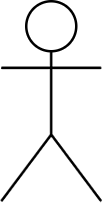
\includegraphics[scale=.1]{Capitulo3/img/actor.png} Ingresa el actor a la aplicación móvil, en el caso del administrador ingresa al portal web mediante una dirección eletrónica.}
  \item {
\includegraphics[scale=.05]{Capitulo3/img/proceso.png} Se muestar la vista IU Inicio. \hyperref[cu2_ta_a]{[Trayectoria alternativa A]}}
  \item {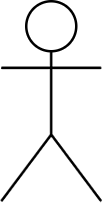
\includegraphics[scale=.1]{Capitulo3/img/actor.png} Selecciona el usuario la opción de \textit{¿Eres nuevo aquí?}}
  \item {
\includegraphics[scale=.05]{Capitulo3/img/proceso.png} Se muestar la vista IU Registro.}
  \item {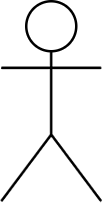
\includegraphics[scale=.1]{Capitulo3/img/actor.png} El actor ingresa los campos requeridos.}
  \item {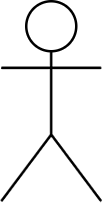
\includegraphics[scale=.1]{Capitulo3/img/actor.png} Presiona el botón para solicitar su registro al sistema.}
  \item {
\includegraphics[scale=.05]{Capitulo3/img/proceso.png} Verifica que el usuario haya ingresado la información requerida como establecido en la \hyperref[rnr_04]{RNR 04}. \hyperref[cu2_ta_b]{[Trayectoria alternativa B]}}
  \item {
\includegraphics[scale=.05]{Capitulo3/img/proceso.png} Verifica que la dirección de correo electrónico cumpla con la RNO. \hyperref[cu2_ta_c]{[Trayectoria alternativa C]}}
  \item {
\includegraphics[scale=.05]{Capitulo3/img/proceso.png} Verifica que la contraseña cumpla con la RNO. \hyperref[cu2_ta_d]{[Trayectoria alternativa D]}}
  \item {
\includegraphics[scale=.05]{Capitulo3/img/proceso.png} Verifica que la contraseña de confirmación coincida con la contrasea ingresada. \hyperref[cu2_ta_e]{[Trayectoria alternativa E]}}
  \item {
\includegraphics[scale=.05]{Capitulo3/img/proceso.png} Verifica que el nombre cumpla con la RNO. \hyperref[cu2_ta_f]{[Trayectoria alternativa F]} \hyperref[cu2_ta_g]{[Trayectoria alternativa G]}}
  \item {
\includegraphics[scale=.05]{Capitulo3/img/proceso.png} Verifica que el apellido paterno cumpla con la RNO. \hyperref[cu2_ta_h]{[Trayectoria alternativa H]} \hyperref[cu2_ta_i]{[Trayectoria alternativa I]}}
  \item {
\includegraphics[scale=.05]{Capitulo3/img/proceso.png} Verifica que el apellido materno cumpla con la RNO. \hyperref[cu2_ta_h]{[Trayectoria alternativa H]} \hyperref[cu2_ta_i]{[Trayectoria alternativa I]}}
  \item {
\includegraphics[scale=.05]{Capitulo3/img/proceso.png} Verifica que el telefóno cumpla con la RN. \hyperref[cu2_ta_j]{[Trayectoria alternativa J]}}
  \item {
\includegraphics[scale=.05]{Capitulo3/img/proceso.png} Verifica que el telefóno cumpla con la RN. \hyperref[cu2_ta_j]{[Trayectoria alternativa J]}}
  \item {
\includegraphics[scale=.05]{Capitulo3/img/proceso.png} Se muestra el mensaje MSG que indica el registro exitoso al sistema.}
  \item {
\includegraphics[scale=.1]{Capitulo3/img/proceso.png} Se redirecciona a la vista IU Confirma tu cuenta.}\\
  \textit{Fin de caso de uso} \\	
\end{enumerate}

\textbf{Trayectoria alternativa A} \phantomsection\label{cu2_ta_a} \\
\textbf{Condición:} El actor presiona la opción de \textit{Iniciar sesión}.\\
 \begin{enumerate}[label=A\arabic*]
  \item {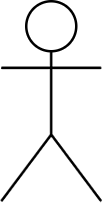
\includegraphics[scale=.1]{Capitulo3/img/actor.png} Presiona el botón de Iniciar sesión.}
  \item {
\includegraphics[scale=.05]{Capitulo3/img/proceso.png} Se muestar la vista IU Iniciar sesión.}
    \item {Continua en el paso 3 de la trayectoria principal.} \\
    \textit{Fin de trayectoria} \\
\end{enumerate}

\textbf{Trayectoria alternativa B} \phantomsection\label{cu2_ta_b} \\
\textbf{Condición:} El actor no proporcionó la información requerida, rompiendo la regla de negocio \hyperref[rnr_04]{RNR 04}.\\
 \begin{enumerate}[label=B\arabic*]
    \item {
\includegraphics[scale=.05]{Capitulo3/img/proceso.png} Muestra el mensaje \hyperref[msja_01]{MSJA 01}, indicando que el actor ha dejado campos en blanco.}
    \item {Continua en el paso 5  de la trayectoria principal.} \\
    \textit{Fin de trayectoria} \\
\end{enumerate}

\textbf{Trayectoria alternativa C} \phantomsection\label{cu2_ta_c}\\
\textbf{Condición:} El actor no ingreso una dirección de correo electrónico que cumpla con la regla de negocio \hyperref[rnrv_02]{RNRV 02}.\\
 \begin{enumerate}[label=C\arabic*]
    \item {
\includegraphics[scale=.05]{Capitulo3/img/proceso.png} Muestra el mensaje \hyperref[msje_02]{MSJE 02}, indicando que la dirección de correo electrónico no es válida.}
    \item {Continua en el paso 5 de la trayectoria principal.} \\
    \textit{Fin de trayectoria} \\
\end{enumerate}

\textbf{Trayectoria alternativa D} \phantomsection\label{cu2_ta_d}\\
\textbf{Condición:} El actor ingreso una contraseña incorrecta que no cumple con la regla de negocio \hyperref[rnrv_03]{RNRV 03}.\\
 \begin{enumerate}[label=D\arabic*]
    \item {
\includegraphics[scale=.05]{Capitulo3/img/proceso.png} Muestra el mensaje \hyperref[msje_01]{MSJE 01}, indicando que el actor ha ingresado datos incorrectos.}
    \item {Continua en el paso 5 de la trayectoria principal.} \\
    \textit{Fin de trayectoria} \\
\end{enumerate}

\textbf{Trayectoria alternativa E} \phantomsection\label{cu2_ta_e}\\
\textbf{Condición:} El acto no ingreso la misma contraseña en los campo \textit{Contraseña} y \textit{Confirmar contraseña} coincidan.\\
 \begin{enumerate}[label=E\arabic*]
    \item {
\includegraphics[scale=.05]{Capitulo3/img/proceso.png} Muestra el mensaje \hyperref[msje_04]{MSJE 04}, indicando que las contraseñas no coinciden.}
    \item {Continua en el paso 5 de la trayectoria principal.} \\
    \textit{Fin de trayectoria} \\
\end{enumerate}

\textbf{Trayectoria alternativa F} \phantomsection\label{cu2_ta_f}\\
\textbf{Condición:} El actor no ingreso un nombre que cumpla con la longitud establecida en la \hyperref[rnl_02]{RNL 02}.\\
 \begin{enumerate}[label=F\arabic*]
    \item {
\includegraphics[scale=.05]{Capitulo3/img/proceso.png} Muestra el mensaje \hyperref[msje_05]{MSJE 05}, indicando que el nombre sobrepasa la longitud máxima.}
    \item {Continua en el paso 5 de la trayectoria principal.} \\
    \textit{Fin de trayectoria} \\
\end{enumerate}

\textbf{Trayectoria alternativa G} \phantomsection\label{cu2_ta_g}\\
\textbf{Condición:} El actor ingreso un nombre que contiene símbolos o carácteres de tipo númericos.\\
 \begin{enumerate}[label=G\arabic*]
    \item {
\includegraphics[scale=.05]{Capitulo3/img/proceso.png} Muestra el mensaje \hyperref[msje_06]{MSJE 06}, indicando que el nombre contiene carácteres de tipo númerico o símbolos.}
    \item {Continua en el paso 5 de la trayectoria principal.} \\
    \textit{Fin de trayectoria} \\
\end{enumerate}

\textbf{Trayectoria alternativa H} \phantomsection\label{cu2_ta_h}\\
\textbf{Condición:} El actor no ingreso un apellido que cumpla con la longitud establecida en la \hyperref[rnl_03]{RNL 03} .\\
 \begin{enumerate}[label=H\arabic*]
    \item {
\includegraphics[scale=.05]{Capitulo3/img/proceso.png} Muestra el mensaje \hyperref[msje_05]{MSJE 05}, indicando que alguno de los apellidos sobrepasa la longitud máxima.}
    \item {Continua en el paso 5 de la trayectoria principal.} \\
    \textit{Fin de trayectoria} \\
\end{enumerate}

\textbf{Trayectoria alternativa I} \phantomsection\label{cu2_ta_i}\\
\textbf{Condición:} El actor ingreso un apellido que contiene símbolos o carácteres de tipo númericos.\\
 \begin{enumerate}[label=I\arabic*]
    \item {
\includegraphics[scale=.05]{Capitulo3/img/proceso.png} Muestra el mensaje \hyperref[msje_06]{MSJE 06}, indicando que el apellido contiene carácteres de tipo númerico o símbolos.}
    \item {Continua en el paso 5 de la trayectoria principal.} \\
    \textit{Fin de trayectoria} \\
\end{enumerate}

\textbf{Trayectoria alternativa J} \phantomsection\label{cu2_ta_j}\\
\textbf{Condición:} El actor ingreso telefóno que no coincide con la longitud establecida en la \hyperref[rnrv_05]{RNRV 05} y \hyperref[rnrv_06]{RNRV 06}.\\
 \begin{enumerate}[label=J\arabic*]
    \item {
\includegraphics[scale=.05]{Capitulo3/img/proceso.png} Muestra el mensaje \hyperref[msje_07]{MSJE 07}, indicando que la longitud del número celular es inválida.}
    \item {Continua en el paso 5 de la trayectoria principal.} \\
    \textit{Fin de trayectoria} \\
\end{enumerate}

\textbf{Trayectoria alternativa K} \phantomsection\label{cu2_ta_k}\\
\textbf{Condición:} El actor ingreso una fecha de nacimiento que no cumple con la \hyperref[rnrv_04]{RNRV 08}.\\
 \begin{enumerate}[label=K\arabic*]
    \item {
\includegraphics[scale=.05]{Capitulo3/img/proceso.png} Muestra el mensaje \hyperref[msje_07]{MSJE 07}, indicando que la longitud del número celular es inválida.}
    \item {Continua en el paso 5 de la trayectoria principal.} \\
    \textit{Fin de trayectoria} \\
\end{enumerate}

\textbf{Trayectoria alternativa } \phantomsection\label{cu2_ta_}\\
\textbf{Condición:} El actor selecciono la opción de \textit{¿Has olvidado tu contraseña?}.\\
 \begin{enumerate}[label=\arabic*]
    \item {
\includegraphics[scale=.05]{Capitulo3/img/proceso.png} Se ejecuta el \hyperref[cu1_1]{CU 1.1 Recuperar contraseña}} \\
    \textit{Fin de trayectoria} \\
\end{enumerate}

\textbf{Trayectoria alternativa } \phantomsection\label{cu2_ta_}\\
\textbf{Condición:} El actor selecciono la opción de \textit{¿Ya tienes una cuenta?}.\\
 \begin{enumerate}[label=\arabic*]
    \item {
\includegraphics[scale=.05]{Capitulo3/img/proceso.png} Se ejecuta el \hyperref[cu1]{CU 1 Iniciar sesión.}}\\
    \textit{Fin de trayectoria} \\
\end{enumerate}

\subsubsection{Puntos de extensión}
\noindent \textbf{Causa de la extensión:} El actor, de tipo de Usuario o Sub-Usuario, selecciono \textit{¿Has olvidado tu contraseña?} \\
\textbf{Región de la trayectoria:} \hyperref[cu2_ta_i]{Trayectoria alternativa I} \\
\textbf{Extiende a:} \hyperref[cu1_1]{CU 1.1 Recuperar contraseña} \\ \par

\noindent \textbf{Causa de la extensión:} El actor, de tipo de Usuario o Sub-Usuario, selecciono \textit{¿Ya tienes una cuenta?} \\
\textbf{Región de la trayectoria:} \hyperref[cu2_ta_j]{Trayectoria alternativa J} \\
\textbf{Extiende a:} \hyperref[cu1]{CU 1 Iniciar sesión}
